\documentclass[11pt, a4paper]{article}

% --- PREAMBLE ---
% Set up packages for math, code, graphics, and layout
\usepackage[utf8]{inputenc}
\usepackage[T1]{fontenc}
\usepackage{lmodern}
\usepackage[margin=1.5in]{geometry}
\usepackage{amsmath}
\usepackage{amssymb}
\usepackage{graphicx}
\usepackage{hyperref}
\usepackage{xcolor}
\usepackage{listings}
\usepackage{palatino}
\usepackage{mathpazo}
\usepackage{microtype}

% Remove paragraph indentation
\setlength{\parindent}{0pt}

% Define colors for code listings
\definecolor{codegreen}{rgb}{0,0.6,0}
\definecolor{codegray}{rgb}{0.5,0.5,0.5}
\definecolor{codepurple}{rgb}{0.58,0,0.82}
\definecolor{backcolour}{rgb}{0.95,0.95,0.95}

% Configure the 'listings' package for C++
\lstdefinestyle{mystyle}{
    backgroundcolor=\color{backcolour},   
    commentstyle=\color{codegreen},
    keywordstyle=\color{magenta},
    numberstyle=\tiny\color{codegray},
    stringstyle=\color{codepurple},
    basicstyle=\ttfamily\footnotesize,
    breakatwhitespace=false,         
    breaklines=true,                 
    captionpos=b,                    
    keepspaces=true,                 
    numbers=left,                    
    numbersep=5pt,                  
    showspaces=false,                
    showstringspaces=false,
    showtabs=false,                  
    tabsize=2,
    language=C++,
    morecomment=[l]{//},
    morecomment=[s]{/*}{*/}
}
\lstset{style=mystyle}

% Improve hyphenation and line breaking
\tolerance=2000
\emergencystretch=3em
\hfuzz=0.5pt

% Setup for the title page
\title{Programming Techniques for Scientific Simulations I: \\ Advanced C++ Optimization Techniques \\ A Comprehensive Textbook}
\author{Based on lecture slides}
\date{\today}

% Hyperlink setup
\hypersetup{
    colorlinks=true,
    linkcolor=blue,
    filecolor=magenta,      
    urlcolor=cyan,
    pdftitle={Programming Techniques for Scientific Simulations - C++ Optimization},
    pdfpagemode=FullScreen,
}

% --- DOCUMENT START ---
\begin{document}

\maketitle
\tableofcontents
\newpage

\section{Introduction: The Quest for High-Performance C++ Code}

In the realm of scientific computing and high-performance simulations, the choice of programming language and optimization techniques can mean the difference between results that take minutes or weeks to compute. C++ has emerged as one of the dominant languages for scientific simulations, not merely because of its inherent performance characteristics, but due to its sophisticated facilities for \textbf{zero-cost abstractions}---the ability to write elegant, maintainable code that, when properly optimized, performs as efficiently as hand-written low-level code.

This textbook chapter explores a collection of advanced C++ optimization techniques that are essential for writing efficient scientific simulation code. While previous material has covered general optimization principles applicable to any programming language---such as algorithmic complexity analysis, cache-aware programming, data structure selection, and memory access patterns---this chapter focuses specifically on \textbf{C++-specific optimizations}. These are techniques that leverage unique features of the C++ language, particularly its powerful template system, to achieve performance that would be difficult or impossible to obtain in other languages.

The techniques we will explore include:

\begin{itemize}
    \item \textbf{Inlining}: A fundamental optimization that eliminates function call overhead by replacing calls with the function's actual code.
    \item \textbf{Copy Elision and Return Value Optimization (RVO/NRVO)}: Compiler optimizations that eliminate unnecessary object copies during return operations.
    \item \textbf{Template Metaprogramming (TMP)}: The technique of performing computations at compile-time using C++'s template system.
    \item \textbf{Lazy Evaluation}: Postponing computations until their results are actually needed, avoiding unnecessary intermediate calculations.
    \item \textbf{Expression Templates}: An advanced technique that combines template metaprogramming with lazy evaluation to optimize mathematical expressions on vectors and matrices.
\end{itemize}

These techniques share a common goal: to allow programmers to write code that is both \textit{expressive} (easy to read, understand, and maintain) and \textit{performant} (executing with minimal overhead and maximum efficiency). The beauty of modern C++ is that we need not sacrifice one for the other.

Throughout this chapter, we will build intuition for these concepts through detailed explanations, practical examples, and step-by-step walkthroughs of how the compiler transforms high-level code into efficient machine instructions. By the end, you will understand not only \textit{how} these optimizations work, but \textit{why} they are structured the way they are, and how to apply them in your own scientific computing projects.

\section{Function Inlining: Eliminating Call Overhead}

\subsection{Understanding Function Call Overhead}

Before we can appreciate the value of inlining, we must first understand what happens when a function is called in a typical compiled program. A function call is not a "free" operation---it involves several steps that consume both time and memory:

\begin{enumerate}
    \item \textbf{Parameter Passing}: Arguments must be placed in the appropriate locations (registers or stack) according to the calling convention.
    \item \textbf{Stack Frame Creation}: The program must save the current instruction pointer (return address) and possibly other register values.
    \item \textbf{Jump to Function}: The instruction pointer must jump to the beginning of the function's code.
    \item \textbf{Function Execution}: The function's body executes.
    \item \textbf{Return Value Handling}: Any return value must be placed in the appropriate location.
    \item \textbf{Stack Frame Destruction}: The saved state must be restored.
    \item \textbf{Return Jump}: Control must return to the calling location.
\end{enumerate}

For large functions that perform significant computation, this overhead is negligible---a few dozen processor cycles among thousands or millions. However, consider a scenario common in scientific computing: a small mathematical function called millions of times in a tight loop. For example:

\begin{lstlisting}[language=C++, caption={A simple function called repeatedly in a loop}]
double square(double x) {
    return x * x;
}

// Called millions of times
for (int i = 0; i < 10000000; ++i) {
    result += square(data[i]);
}
\end{lstlisting}

In this case, the function \texttt{square()} performs a single multiplication, which on modern processors takes only a few cycles. However, the overhead of calling the function---parameter passing, jumping, returning---might take 10-20 cycles or more. The overhead dominates the actual work!

This is where \textbf{inlining} becomes critical.

\subsection{What is Inlining?}

\textbf{Inlining} is an optimization where the compiler replaces a function call with the function's actual code. Instead of jumping to a separate location, executing code, and returning, the compiler inserts the function's body directly at the call site.

The \texttt{inline} keyword in C++ serves as a \textit{suggestion} to the compiler that a particular function should be inlined. The syntax is straightforward:

\begin{lstlisting}[language=C++, caption={Declaring an inline function}]
inline double square(double x) {
    return x * x;
}
\end{lstlisting}

When the compiler sees a call to \texttt{square()}, instead of generating a function call, it generates code equivalent to:

\begin{lstlisting}[language=C++, caption={Conceptual transformation after inlining}]
for (int i = 0; i < 10000000; ++i) {
    result += data[i] * data[i];  // Function body inserted directly
}
\end{lstlisting}

\subsection{Benefits of Inlining}

The advantages of inlining extend beyond merely eliminating call overhead:

\begin{enumerate}
    \item \textbf{Elimination of Call/Return Overhead}: The most obvious benefit---no parameter passing, no stack frame manipulation, no jumps.
    
    \item \textbf{Enabling Secondary Optimizations}: When the compiler sees the complete code in context, it can perform optimizations that would be impossible across function boundaries. For example:
    \begin{itemize}
        \item Constant folding: If arguments are constants, the compiler can compute the result at compile time.
        \item Dead code elimination: If parts of the inlined code are never used, they can be removed.
        \item Register allocation: Variables can be kept in registers without saving/restoring across calls.
        \item Common subexpression elimination: Repeated calculations can be identified and eliminated.
    \end{itemize}
    
    \item \textbf{Improved Instruction Cache Locality}: Instead of jumping to different code locations, all relevant code is contiguous, improving cache performance.
\end{enumerate}

\subsection{Important Caveats and Modern Compiler Behavior}

While the \texttt{inline} keyword exists in C++, it's crucial to understand its limitations and modern interpretation:

\begin{itemize}
    \item \textbf{It's a Suggestion, Not a Command}: The compiler is free to ignore the \texttt{inline} keyword. If a function is large, complex, or recursive, the compiler may choose not to inline it.
    
    \item \textbf{Compilers Inline Without Being Asked}: Modern optimizing compilers (GCC, Clang, MSVC with optimization flags like \texttt{-O2}, \texttt{-O3}) perform automatic inlining based on sophisticated heuristics. They may inline functions not marked \texttt{inline} if they determine it's beneficial.
    
    \item \textbf{The ODR (One Definition Rule) Exception}: The primary modern use of the \texttt{inline} keyword is actually to allow multiple definitions of the same function across translation units without violating the One Definition Rule. This is why functions defined in header files are typically marked \texttt{inline}.
    
    \item \textbf{Trade-offs}: Excessive inlining can increase code size (code bloat), potentially harming instruction cache performance. The compiler must balance these concerns.
\end{itemize}

For scientific computing, where small mathematical functions are called repeatedly, inlining is not just an optimization---it's often essential for achieving competitive performance.

\subsection{Example: Measuring the Impact of Inlining}

Consider a practical experiment comparing inlined and non-inlined versions of a simple function:

\begin{lstlisting}[language=C++, caption={Comparing inlined and non-inlined functions}]
#include <iostream>
#include <chrono>
#include <vector>

// Non-inlined version (using noinline attribute to force this)
__attribute__((noinline))
double square_noinline(double x) {
    return x * x;
}

// Inlined version
inline double square_inline(double x) {
    return x * x;
}

int main() {
    const int N = 100000000;
    std::vector<double> data(N, 2.5);
    double result = 0.0;
    
    // Test non-inlined version
    auto start = std::chrono::high_resolution_clock::now();
    for (int i = 0; i < N; ++i) {
        result += square_noinline(data[i]);
    }
    auto end = std::chrono::high_resolution_clock::now();
    auto duration_noinline = std::chrono::duration_cast<std::chrono::milliseconds>(end - start);
    
    result = 0.0;
    
    // Test inlined version
    start = std::chrono::high_resolution_clock::now();
    for (int i = 0; i < N; ++i) {
        result += square_inline(data[i]);
    }
    end = std::chrono::high_resolution_clock::now();
    auto duration_inline = std::chrono::duration_cast<std::chrono::milliseconds>(end - start);
    
    std::cout << "Non-inlined: " << duration_noinline.count() << " ms\n";
    std::cout << "Inlined: " << duration_inline.count() << " ms\n";
    std::cout << "Speedup: " << (double)duration_noinline.count() / duration_inline.count() << "x\n";
    
    return 0;
}
\end{lstlisting}

On most modern systems with optimization enabled, the inlined version will be significantly faster, often by a factor of 2-5x or more for such simple operations.

For further detailed information on the \texttt{inline} specifier, its semantics, and its evolution in different C++ standards, consult the comprehensive reference at \url{https://en.cppreference.com/w/cpp/language/inline}.

\section{Copy Elision and Return Value Optimization}

\subsection{The Problem: Expensive Object Returns}

In C++, objects can be returned from functions by value. Before modern optimizations, this operation was notoriously expensive for large objects. Consider what happens when you write:

\begin{lstlisting}[language=C++, caption={Returning an object by value}]
std::vector<int> create_vector() {
    std::vector<int> v{1, 2, 3, 4, 5};
    return v;
}

int main() {
    std::vector<int> result = create_vector();
}
\end{lstlisting}

Without optimization, the sequence of operations would be:

\begin{enumerate}
    \item \textbf{Inside \texttt{create\_vector()}}: Construct the local vector \texttt{v} with 5 elements.
    \item \textbf{Return Statement}: Create a temporary copy of \texttt{v} (copy constructor called).
    \item \textbf{After Return}: The local \texttt{v} is destroyed (destructor called).
    \item \textbf{In \texttt{main()}}: The temporary is used to initialize \texttt{result} (copy or move constructor called).
    \item \textbf{Cleanup}: The temporary is destroyed (destructor called).
\end{enumerate}

For a vector containing thousands of elements, this involves multiple memory allocations, data copying, and deallocations---extremely expensive operations.

\subsection{Copy Elision: The Solution}

\textbf{Copy elision} is a compiler optimization that eliminates these unnecessary copy and move operations. Instead of creating the object in one location and copying it to another, the compiler constructs the object directly in its final destination.

The C++ standard explicitly \textit{allows} copy elision, even if the copy or move constructor has observable side effects (such as printing to console or logging). This is unusual---most optimizations are forbidden if they change observable behavior, but copy elision is considered so important that it's permitted to "skip" constructor calls.

\subsection{Return Value Optimization (RVO)}

\textbf{Return Value Optimization (RVO)} is a specific form of copy elision that applies when returning a temporary (unnamed) object:

\begin{lstlisting}[language=C++, caption={RVO example with temporary object}]
std::vector<int> create_vector() {
    return std::vector<int>{1, 2, 3, 4, 5};  // Temporary object
}
\end{lstlisting}

Here, instead of constructing the temporary inside \texttt{create\_vector()}, copying it to the return location, and destroying the temporary, the compiler constructs the vector directly in the location where \texttt{result} will exist in the calling function.

\textbf{Important}: As of C++17, RVO is \textit{mandatory} in many cases. The compiler must perform this optimization; it's not optional.

\subsection{Named Return Value Optimization (NRVO)}

\textbf{Named Return Value Optimization (NRVO)} extends RVO to named local variables:

\begin{lstlisting}[language=C++, caption={NRVO example with named local object}]
std::vector<int> create_vector() {
    std::vector<int> v{1, 2, 3, 4, 5};  // Named local variable
    // ... potentially do some operations on v ...
    return v;
}
\end{lstlisting}

NRVO is more complex than RVO because the named object \texttt{v} might be returned from multiple paths in the function, making it harder for the compiler to guarantee that it can construct \texttt{v} directly in the caller's location. Therefore, while NRVO is commonly performed by modern compilers, it's not mandatory (even in C++17), and there are cases where it cannot be applied.

\subsection{Observing Copy Elision in Practice}

Let's create a demonstration that shows when copy elision occurs:

\begin{lstlisting}[language=C++, caption={Demonstrating copy elision with observable constructors}]
#include <iostream>

struct C {
    C() { 
        std::cout << "C constructor\n"; 
    }
    
    C(const C& c) { 
        std::cout << "C copy constructor\n"; 
    }
    
    ~C() {
        std::cout << "C destructor\n";
    }
};

// RVO case: returning temporary
C f() {
    return C();
}

// NRVO case: returning named object
C g() {
    C c;
    return c;
}

int main() {
    std::cout << "Creating c1 with RVO:\n";
    C c1 = f();
    
    std::cout << "\nCreating c2 with NRVO:\n";
    C c2 = g();
    
    std::cout << "\nLeaving main (destructors called):\n";
    return 0;
}
\end{lstlisting}

\textbf{Expected output with optimization enabled (C++17 or later)}:

\begin{verbatim}
Creating c1 with RVO:
C constructor

Creating c2 with NRVO:
C constructor

Leaving main (destructors called):
C destructor
C destructor
\end{verbatim}

Notice that the copy constructor is never called! Both \texttt{c1} and \texttt{c2} are constructed directly in their final locations.

\subsection{Experimenting with Compiler Flags}

To truly understand copy elision, you should compile the above program with different compiler flags:

\begin{itemize}
    \item \texttt{g++ -std=c++17 -O2 test.cpp}: Full optimization, C++17 standard (RVO mandatory, NRVO likely)
    \item \texttt{g++ -std=c++14 -O0 test.cpp}: No optimization, C++14 (copy elision possible but less likely)
    \item \texttt{g++ -std=c++17 -O2 -fno-elide-constructors test.cpp}: Explicitly disable copy elision (useful for comparison)
\end{itemize}

With \texttt{-fno-elide-constructors}, you'll see copy constructors being called, demonstrating the overhead that copy elision eliminates.

\subsection{Implications for Scientific Computing}

For scientific computing, copy elision is crucial when working with large data structures:

\begin{itemize}
    \item \textbf{Large matrices or vectors}: Returning these by value would be prohibitively expensive without copy elision.
    \item \textbf{Complex result objects}: Functions can naturally return complete result objects without performance penalty.
    \item \textbf{Clean API design}: You can design intuitive interfaces that return objects by value, knowing the compiler will optimize away unnecessary copies.
\end{itemize}

The comprehensive reference for copy elision can be found at \url{https://en.cppreference.com/w/cpp/language/copy_elision}.

\section{Template Metaprogramming: Computation at Compile Time}

\subsection{What is "Meta"?}

Before diving into template metaprogramming, we must understand the concept of "meta." The prefix \textbf{"meta-"} comes from Greek and means "beyond," "about," or "at a higher level."

In computing, "meta" refers to operating at one level of abstraction above the primary level:

\begin{itemize}
    \item \textbf{Metasyntax}: Syntax for describing syntax itself (e.g., Backus-Naur Form describes the syntax of programming languages)
    \item \textbf{Metalanguage}: A language used to describe or discuss another language (e.g., English used to discuss French grammar)
    \item \textbf{Metadata}: Data about data (e.g., a file's creation date, size, and author are metadata about the file's content)
    \item \textbf{Metareasoning}: Reasoning about reasoning itself (e.g., analyzing how you solve problems)
\end{itemize}

Therefore, a \textbf{metaprogram} is a program that operates on programs---it writes, analyzes, or transforms programs.

\subsection{The C++ Compiler as a Turing Machine}

In 1994, Erwin Unruh made a groundbreaking discovery: the C++ template system is \textbf{Turing complete}. This means that the template instantiation mechanism itself can perform any computation that a classical computer can perform.

This has profound implications:

\begin{enumerate}
    \item \textbf{Arbitrary Compile-Time Computation}: You can perform complex calculations during compilation, with results embedded directly in the executable.
    
    \item \textbf{Compile-Time Loops}: Through template recursion, you can achieve loop-like behavior at compile time.
    
    \item \textbf{Compile-Time Conditionals}: Using template specialization, you can implement branching logic during compilation.
    
    \item \textbf{Undecidable Halting Problem}: Just like with regular programs, it's impossible to determine in general whether template instantiation will ever complete. You can write template code that causes the compiler to recurse infinitely (until it hits instantiation depth limits and gives up).
\end{enumerate}

This capability is formally called \textbf{Template Metaprogramming (TMP)}.

\subsection{Erwin Unruh's Historic Prime Number Program}

To demonstrate the Turing completeness of C++ templates, Unruh wrote a program that computes prime numbers \textit{during compilation} and outputs them as compiler error messages. While the original 1994 program no longer compiles with modern compilers (due to changes in error message formatting), updated versions demonstrate the same principle.

Here's a conceptual understanding of the approach:

\begin{lstlisting}[language=C++, caption={Simplified prime number metaprogram concept}]
// Check if p is prime by testing divisibility from i down to 2
template<int p, int i> 
struct is_prime {
    enum { 
        prim = (p % i) && is_prime<(i > 2 ? p : 0), i-1>::prim 
    };
};

// Base case: stop recursion
template<> 
struct is_prime<0, 0> { 
    enum { prim = 1 }; 
};

// Print prime numbers (causes compilation errors for primes)
template<int i> 
struct Prime_print {
    Prime_print<i-1> a;  // Recursive instantiation
    enum { prim = is_prime<i, i-1>::prim };
    void f() { 
        D<i> d = prim;  // This line causes an error if i is prime
    }
};
\end{lstlisting}

The program uses template recursion to check each number for primality. For prime numbers, it triggers a specific type conversion error that includes the number in the error message. The compiler essentially executes a prime-finding algorithm while trying to compile the code!

To compile the modern version:

\begin{verbatim}
# GNU compiler
g++ -std=c++03 -fpermissive -DLAST=60 unruh_new.cpp 2>&1 | grep "In instantiation"

# Clang compiler
clang++ -std=c++03 -DLAST=60 unruh_new.cpp 2>&1 | grep -i error
\end{verbatim}

This computes all prime numbers up to 60 during compilation!

While this is primarily a curiosity demonstrating the power of templates, it illustrates a fundamental principle we'll exploit: \textit{computations can be moved from runtime to compile time}.

For more information, see Unruh's original work at \url{http://www.erwin-unruh.de/Prim.html}.

\subsection{Factorial: The "Hello World" of Template Metaprogramming}

Just as "Hello World" is the canonical first program in a new language, computing factorial is the canonical introduction to template metaprogramming. It demonstrates the core concepts in their simplest form.

\subsubsection{The Traditional Approach (Enum Version)}

In early C++ (before C++11), in-class initialization of static const members was restricted, so template metaprograms typically used enums:

\begin{lstlisting}[language=C++, caption={Compile-time factorial using enums}]
// General template: factorial of N
template<int N>
struct Factorial {
    enum { value = N * Factorial<N-1>::value };
};

// Specialization: base case to stop recursion
template<>
struct Factorial<1> {
    enum { value = 1 };
};

// Usage
int main() {
    int result = Factorial<5>::value;  // result = 120, computed at compile time!
    return 0;
}
\end{lstlisting}

\subsubsection{Understanding the Mechanism}

Let's trace how the compiler evaluates \texttt{Factorial<5>::value}:

\begin{enumerate}
    \item Compiler encounters \texttt{Factorial<5>::value}
    \item Instantiates \texttt{Factorial<5>}, which requires \texttt{5 * Factorial<4>::value}
    \item Instantiates \texttt{Factorial<4>}, which requires \texttt{4 * Factorial<3>::value}
    \item Instantiates \texttt{Factorial<3>}, which requires \texttt{3 * Factorial<2>::value}
    \item Instantiates \texttt{Factorial<2>}, which requires \texttt{2 * Factorial<1>::value}
    \item Instantiates \texttt{Factorial<1>} (matches specialization), which has \texttt{value = 1}
    \item Unwinds: \texttt{Factorial<2>::value = 2 * 1 = 2}
    \item Unwinds: \texttt{Factorial<3>::value = 3 * 2 = 6}
    \item Unwinds: \texttt{Factorial<4>::value = 4 * 6 = 24}
    \item Unwinds: \texttt{Factorial<5>::value = 5 * 24 = 120}
\end{enumerate}

The key insight: \textit{all of this happens during compilation}! The resulting machine code contains the constant 120 directly---no factorial computation occurs at runtime.

\subsubsection{Modern C++ Approach (Static Const Version)}

Modern C++ allows in-class initialization of static const members, providing cleaner syntax:

\begin{lstlisting}[language=C++, caption={Modern compile-time factorial using static const}]
template<int N>
struct Factorial {
    static const int value = N * Factorial<N-1>::value;
};

template<>
struct Factorial<1> {
    static const int value = 1;
};

// Or using constexpr (C++11 and later)
template<int N>
struct Factorial {
    static constexpr int value = N * Factorial<N-1>::value;
};

template<>
struct Factorial<1> {
    static constexpr int value = 1;
};
\end{lstlisting}

Both versions produce identical results, but \texttt{constexpr} more explicitly communicates that these are compile-time constants.

\subsubsection{Visualizing the Generated Code}

To truly understand what the compiler produces, visit \url{https://cppinsights.io/} and paste the factorial code. C++ Insights shows you the code after template instantiation. You'll see that the compiler has generated concrete structs with specific integer values---essentially "baking in" the computed factorial.

\subsubsection{Why This Matters for Scientific Computing}

Template metaprogramming allows us to:

\begin{itemize}
    \item \textbf{Compute Constants}: Mathematical constants or lookup tables can be generated at compile time.
    \item \textbf{Generate Optimized Code}: Different code paths for different sizes, types, or configurations.
    \item \textbf{Unroll Loops}: As we'll see next, loops can be unrolled to eliminate overhead for small, fixed-size operations.
\end{itemize}

\section{Unrolling Loops with Template Metaprogramming}

\subsection{The Performance Problem: Loop Overhead in Small Vectors}

Consider one of the most fundamental operations in scientific computing: the \textbf{dot product} (also called scalar product or inner product) of two vectors:

\begin{equation}
\text{dot}(\mathbf{a}, \mathbf{b}) = \sum_{i=0}^{N-1} a_i \cdot b_i = a_0 b_0 + a_1 b_1 + \cdots + a_{N-1} b_{N-1}
\end{equation}

A straightforward implementation looks like this:

\begin{lstlisting}[language=C++, caption={Standard dot product implementation}]
double dot(const double* a, const double* b, int N) {
    double result = 0.0;
    for (int i = 0; i < N; ++i) {
        result += a[i] * b[i];
    }
    return result;
}
\end{lstlisting}

This seems optimal---each iteration performs one multiplication and one addition, which are the fundamental operations required. However, there's hidden overhead in the loop itself:

\begin{enumerate}
    \item Initialize loop counter \texttt{i = 0}
    \item Compare \texttt{i < N}
    \item Increment \texttt{i++}
    \item Branch (conditional jump) to continue or exit the loop
    \item Potential branch misprediction penalties
\end{enumerate}

For large vectors (N > 100), this overhead is negligible---a few dozen cycles among thousands. But for \textit{small} vectors, common in many applications (3D coordinates, 4x4 transformation matrices, small state vectors), the overhead dominates the actual computation.

\subsection{Performance Analysis: When Loop Overhead Dominates}

\begin{figure}[h!]
\centering
\includegraphics[width=0.7\textwidth]{placeholder_dot_product_performance_graph.png}
\caption{Performance of the standard dot product function as vector length increases. For small vectors (N < 10), performance is far below peak due to loop overhead. Performance only approaches peak around N = 100. The y-axis shows performance in MFlops (millions of floating-point operations per second), while the x-axis shows vector length. Source: Todd Veldhuizen, "Techniques for Scientific C++", Indiana University Computer Science Technical Report \#542, 2000.}
\end{figure}

The graph from the slides reveals a striking pattern:

\begin{itemize}
    \item \textbf{Small vectors (N < 10)}: Achieving only 20-30\% of peak performance
    \item \textbf{Medium vectors (N = 10-50)}: Gradually improving performance
    \item \textbf{Large vectors (N > 100)}: Approaching peak performance (70+ MFlops)
\end{itemize}

\textbf{Why the poor performance for small vectors?}

For a 3-element dot product:
\begin{itemize}
    \item \textbf{Useful operations}: 3 multiplications + 2 additions = 5 floating-point operations
    \item \textbf{Loop overhead}: 3 comparisons + 3 increments + 3 branches $\approx$ 15-20 operations
\end{itemize}

The overhead is 3-4 times the actual work! This is unacceptable for performance-critical code.

\subsection{The Solution: Unrolled Loops}

For fixed-size vectors, we can eliminate the loop entirely by writing out each operation explicitly:

\begin{lstlisting}[language=C++, caption={Hand-unrolled dot product for 3D vectors}]
inline double dot3(const double* a, const double* b) {
    return a[0]*b[0] + a[1]*b[1] + a[2]*b[2];
}
\end{lstlisting}

This version:
\begin{itemize}
    \item Has \textbf{zero loop overhead}
    \item Allows the compiler to see all operations simultaneously, enabling aggressive optimization
    \item Can be transformed into SIMD (Single Instruction, Multiple Data) instructions by modern compilers
    \item Achieves near-peak performance immediately
\end{itemize}

\subsection{The Challenge: Generic Unrolling}

The problem is scalability. We could write:

\begin{lstlisting}[language=C++, caption={Multiple hand-written versions---not maintainable}]
inline double dot2(const double* a, const double* b) {
    return a[0]*b[0] + a[1]*b[1];
}

inline double dot3(const double* a, const double* b) {
    return a[0]*b[0] + a[1]*b[1] + a[2]*b[2];
}

inline double dot4(const double* a, const double* b) {
    return a[0]*b[0] + a[1]*b[1] + a[2]*b[2] + a[3]*b[3];
}

// ... and so on for each size we need
\end{lstlisting}

But this is unmaintainable. What if we have a template class like:

\begin{lstlisting}[language=C++, caption={TinyVector template class}]
template<typename T, int N>
class TinyVector {
public:
    T& operator[](int i) { return data[i]; }
    T operator[](int i) const { return data[i]; }
private:
    T data[N];
};
\end{lstlisting}

We want a single \texttt{dot()} function that works for \texttt{TinyVector<double, 3>}, \texttt{TinyVector<double, 4>}, \texttt{TinyVector<float, 16>}, etc., and automatically generates the optimal unrolled code for each size.

\textbf{This is where template metaprogramming saves us.}

\subsection{Unrolled Dot Product via Template Metaprogramming}

The solution uses recursive template instantiation to generate unrolled code at compile time:

\begin{lstlisting}[language=C++, caption={Generic unrolled dot product using templates}]
// Recursive case: process element I and recurse to I-1
template<int I>
struct meta_dot {
    template<typename T, int N>
    static T f(TinyVector<T,N>& a, TinyVector<T,N>& b) {
        return a[I]*b[I] + meta_dot<I-1>::f(a,b);
    }
};

// Base case: process element 0 and stop recursion
template<>
struct meta_dot<0> {
    template<typename T, int N>
    static T f(TinyVector<T,N>& a, TinyVector<T,N>& b) {
        return a[0]*b[0];
    }
};

// User-facing function: kick off the metaprogram
template<typename T, int N>
inline T dot(TinyVector<T,N>& a, TinyVector<T,N>& b) {
    return meta_dot<N-1>::f(a,b);
}
\end{lstlisting}

\subsection{Step-by-Step: How the Compiler Processes This}

Let's trace what happens when you write:

\begin{lstlisting}[language=C++]
TinyVector<double, 4> a, b;
double r = dot(a, b);
\end{lstlisting}

\textbf{Step 1}: Call \texttt{dot(a, b)}
\begin{lstlisting}[language=C++]
// T=double, N=4
return meta_dot<N-1>::f(a,b);  // Instantiate meta_dot<3>
\end{lstlisting}

\textbf{Step 2}: Instantiate \texttt{meta\_dot<3>::f}
\begin{lstlisting}[language=C++]
return a[3]*b[3] + meta_dot<2>::f(a,b);  // Instantiate meta_dot<2>
\end{lstlisting}

\textbf{Step 3}: Instantiate \texttt{meta\_dot<2>::f}
\begin{lstlisting}[language=C++]
return a[2]*b[2] + meta_dot<1>::f(a,b);  // Instantiate meta_dot<1>
\end{lstlisting}

\textbf{Step 4}: Instantiate \texttt{meta\_dot<1>::f}
\begin{lstlisting}[language=C++]
return a[1]*b[1] + meta_dot<0>::f(a,b);  // Instantiate meta_dot<0>
\end{lstlisting}

\textbf{Step 5}: Instantiate \texttt{meta\_dot<0>::f} (specialization matches!)
\begin{lstlisting}[language=C++]
return a[0]*b[0];  // Base case: no further recursion
\end{lstlisting}

\textbf{Step 6}: Compiler substitutes everything back:
\begin{lstlisting}[language=C++]
double r = a[3]*b[3] + a[2]*b[2] + a[1]*b[1] + a[0]*b[0];
\end{lstlisting}

The final generated code is exactly as if we had written the unrolled version by hand!

\subsection{Critical Success Factors}

Two things make this optimization work:

\begin{enumerate}
    \item \textbf{Template Recursion}: The compile-time recursion generates the sequence of operations.
    \item \textbf{Inlining}: All the function calls (\texttt{f()}) must be inlined, or we'd still have call overhead. The \texttt{inline} keyword on the user-facing \texttt{dot()} function helps, and modern compilers will inline the static member functions of \texttt{meta\_dot} automatically.
\end{enumerate}

Without inlining, we'd just have a recursive function with call overhead. With inlining, the recursion disappears entirely, leaving only the arithmetic operations.

\subsection{Generalizing to Other Operations}

The same technique applies to any fixed-size operation:

\begin{itemize}
    \item Vector addition: \texttt{c[i] = a[i] + b[i]} for all i
    \item Vector normalization: compute length, then divide each element
    \item Matrix-vector multiplication: unroll both dimensions
    \item Cross products, quaternion operations, etc.
\end{itemize}

This is the foundation of high-performance small-vector mathematics libraries used throughout computer graphics, physics simulations, and numerical computing.

\section{Expression Templates: Motivation and Problem Statement}

\subsection{Operator Overloading: Convenience vs. Performance}

One of C++'s most powerful features is operator overloading, which allows us to define how operators (+, -, *, /, etc.) work with user-defined types. For vector classes, this enables intuitive mathematical notation:

\begin{lstlisting}[language=C++, caption={Simple vector class with operator overloading}]
template <typename T>
class simplevector {
private:
    T* p_;           // Pointer to data
    size_t sz_;      // Size of vector
    
public:
    explicit simplevector(size_t s = 0);
    simplevector(const simplevector& v);
    ~simplevector();
    
    size_t size() const { return sz_; }
    T& operator[](size_t i) { return p_[i]; }
    const T& operator[](size_t i) const { return p_[i]; }
    
    // Compound assignment
    simplevector& operator+=(const simplevector& v);
    
    // Swap operation
    void swap(simplevector& v) {
        std::swap(p_, v.p_);
        std::swap(sz_, v.sz_);
    }
    
    // Assignment via copy-and-swap idiom
    simplevector& operator=(simplevector v) {
        swap(v);
        return *this;
    }
};

// Free function: binary plus operator
template <typename T>
simplevector<T> operator+(const simplevector<T>& x, 
                          const simplevector<T>& y) {
    simplevector<T> result = x;  // Copy constructor
    result += y;                  // Compound addition
    return result;                // Return by value
}
\end{lstlisting}

This allows beautiful, mathematical code:

\begin{lstlisting}[language=C++, caption={Intuitive vector arithmetic}]
simplevector<double> a(1000), b(1000), c(1000), d(1000);
// ... initialize vectors ...
a = b + c + d;
\end{lstlisting}

However, there's a severe performance problem lurking beneath this elegant interface.

\subsection{The Hidden Cost: Temporary Objects}

Let's analyze what actually happens when we execute \texttt{a = b + c + d}:

\textbf{Evaluation order} (left-to-right, by operator precedence):
\begin{enumerate}
    \item \texttt{tmp1 = b + c}
    \item \texttt{tmp2 = tmp1 + d}
    \item \texttt{a = tmp2}
\end{enumerate}

\textbf{Detailed operation breakdown:}

\textbf{Step 1: \texttt{tmp1 = b + c}}
\begin{itemize}
    \item Call \texttt{operator+(b, c)}
    \item Inside operator+: Create \texttt{result} by copying \texttt{b} (allocate N doubles, copy N values)
    \item Call \texttt{result += c} (loop through N elements, N additions, write N values)
    \item Return \texttt{result} (copy to \texttt{tmp1})
    \item Destroy \texttt{result}
\end{itemize}
\textbf{Operations:} 3N reads + 2N writes + 1 allocation + 1 deallocation

\textbf{Step 2: \texttt{tmp2 = tmp1 + d}}
\begin{itemize}
    \item Call \texttt{operator+(tmp1, d)}
    \item Create \texttt{result} by copying \texttt{tmp1} (allocate N doubles, copy N values)
    \item Call \texttt{result += d} (N additions, N writes)
    \item Return \texttt{result} (copy to \texttt{tmp2})
    \item Destroy \texttt{result}
\end{itemize}
\textbf{Operations:} 3N reads + 2N writes + 1 allocation + 1 deallocation

\textbf{Step 3: \texttt{a = tmp2}}
\begin{itemize}
    \item Call \texttt{operator=(tmp2)}
    \item Using copy-and-swap: copy \texttt{tmp2}, swap with \texttt{a}
    \item Destroy old \texttt{a}
\end{itemize}
\textbf{Operations:} N reads + N writes + 1 allocation + 1 deallocation

\subsection{The Performance Disaster}

\textbf{Total operations for \texttt{a = b + c + d}:}
\begin{itemize}
    \item \textbf{Memory reads:} 3N + 3N + N = 7N
    \item \textbf{Memory writes:} 2N + 2N + N = 5N
    \item \textbf{Allocations/deallocations:} 6 total
\end{itemize}

\textbf{What we actually want} (ideal hand-optimized version):
\begin{lstlisting}[language=C++, caption={Optimal implementation: single pass}]
for (int i = 0; i < N; ++i) {
    a[i] = b[i] + c[i] + d[i];
}
\end{lstlisting}

\textbf{Optimal operations:}
\begin{itemize}
    \item \textbf{Memory reads:} 3N (read b[i], c[i], d[i])
    \item \textbf{Memory writes:} N (write a[i])
    \item \textbf{Allocations/deallocations:} 0
\end{itemize}

\textbf{Overhead ratio:} The naive operator overloading version does approximately \textbf{2.5-3x more memory operations} than necessary, plus allocation overhead!

\subsection{Benchmark Demonstration}

To observe this performance difference, compile and run these tests:

\begin{lstlisting}[language=C++, caption={Benchmark: naive vs. hand-optimized}]
// timesimple.cpp - Naive implementation
simplevector<double> a(N), b(N), c(N), d(N);
a = b + c + d;  // Multiple temporaries

// timesimple_handopt.cpp - Hand-optimized version
simplevector<double> a(N), b(N), c(N), d(N);
for (int i = 0; i < N; ++i) {
    a[i] = b[i] + c[i] + d[i];
}
\end{lstlisting}

Compile and time:
\begin{verbatim}
g++ -O3 -march=native -fopt-info-loop timesimple.cpp -o timesimple
g++ -O3 -march=native -fopt-info-loop timesimple_handopt.cpp -o timesimple_handopt
time -p ./timesimple
time -p ./timesimple_handopt
\end{verbatim}

The hand-optimized version will typically be 2-3x faster, even with full compiler optimization.

For detailed information on evaluation order and operator precedence (which determines how the expression is parsed), see:
\begin{itemize}
    \item \url{https://en.cppreference.com/w/cpp/language/eval_order}
    \item \url{https://en.cppreference.com/w/cpp/language/operator_precedence}
\end{itemize}

\subsection{The Fundamental Goal}

\textbf{What we want:} The elegant syntax of \texttt{a = b + c + d} with the performance of the hand-optimized loop.

\textbf{The solution:} Expression Templates (ET)

Expression templates are a sophisticated technique, developed independently by Todd Veldhuizen and David Vandevoorde in the mid-1990s, that allows us to achieve exactly this. They are now used in virtually every high-performance C++ linear algebra library.

\section{Lazy Evaluation: Postponing Computation}

\subsection{The Core Insight}

The key to expression templates is a simple but powerful idea: \textbf{don't perform the computation immediately---remember what needs to be computed and do it later}.

Consider again:
\begin{lstlisting}[language=C++]
simplevector<double> a(N), b(N), c(N);
a = b + c;
\end{lstlisting}

Current behavior:
\begin{enumerate}
    \item \texttt{operator+(b, c)} is called
    \item Copy \texttt{b} into temporary \texttt{result} (loop 1)
    \item Add \texttt{c} to \texttt{result} (loop 2)
    \item Return \texttt{result}
    \item Assign \texttt{result} to \texttt{a} (loop 3)
\end{enumerate}

\textbf{Three separate loops!}

\textbf{Lazy evaluation approach:}
\begin{enumerate}
    \item \texttt{operator+(b, c)} returns a lightweight object that \textit{describes} "b + c" but doesn't compute it
    \item This description object is passed to \texttt{operator=}
    \item \texttt{operator=} performs the computation in a \textit{single} loop: \texttt{a[i] = b[i] + c[i]}
\end{enumerate}

\textbf{One loop total!}

\subsection{Implementing Lazy Evaluation: The vectorsum Class}

We need a new class that represents "the sum of two vectors" without actually computing it:

\begin{lstlisting}[language=C++, caption={vectorsum: a lazy expression object}]
template <typename T>
class vectorsum {
private:
    const lazyvector<T>& left_;   // Reference to first operand
    const lazyvector<T>& right_;  // Reference to second operand
    
public:
    typedef T value_type;
    typedef unsigned int size_type;
    
    // Constructor: just store references to operands
    vectorsum(const lazyvector<T>& x, const lazyvector<T>& y)
        : left_(x), right_(y) {}
    
    // Subscript: compute on-demand
    value_type operator[](size_type i) const {
        return left_[i] + right_[i];  // Compute when asked!
    }
};
\end{lstlisting}

\textbf{Key points:}
\begin{itemize}
    \item \texttt{vectorsum} stores \textbf{references} to the operands, not copies
    \item It has no data array of its own
    \item \texttt{operator[]} computes the result \textit{on-demand} when called
    \item The object is very lightweight (just two pointers)
\end{itemize}

\subsection{Modified operator+}

Now \texttt{operator+} simply returns a \texttt{vectorsum} object:

\begin{lstlisting}[language=C++, caption={Lazy operator+: no computation performed}]
template <typename T>
inline vectorsum<T> operator+(const lazyvector<T>& x,
                              const lazyvector<T>& y) {
    return vectorsum<T>(x, y);  // Just create description object
}
\end{lstlisting}

This is extremely fast---just construct a small object with two references. No loops, no memory allocation, no computation.

\subsection{Modified Assignment Operator}

The real work happens in assignment:

\begin{lstlisting}[language=C++, caption={Assignment from vectorsum: computation happens here}]
template <typename T>
class lazyvector {
public:
    // Standard assignment
    lazyvector& operator=(const lazyvector& v) { /* ... */ }
    
    // NEW: Assignment from a vectorsum
    lazyvector& operator=(const vectorsum<T>& v) {
        // Single loop: compute directly into this vector
        for (size_type i = 0; i < size(); ++i) {
            p_[i] = v[i];  // Calls vectorsum::operator[], which computes left[i]+right[i]
        }
        return *this;
    }
};
\end{lstlisting}

\subsection{The Complete Evaluation}

When we write:
\begin{lstlisting}[language=C++]
lazyvector<double> a(N), b(N), c(N);
a = b + c;
\end{lstlisting}

Here's what happens:

\textbf{Step 1:} \texttt{operator+(b, c)} is called
\begin{itemize}
    \item Returns \texttt{vectorsum<double>(b, c)}
    \item This is cheap: just store two references
    \item \textbf{No computation yet!}
\end{itemize}

\textbf{Step 2:} \texttt{operator=(vectorsum)} is called
\begin{itemize}
    \item Loop: \texttt{for (i = 0; i < N; ++i)}
    \item Each iteration: \texttt{p\_[i] = v[i]}
    \item \texttt{v[i]} calls \texttt{vectorsum::operator[](i)}
    \item Which returns \texttt{left\_[i] + right\_[i]}
    \item Equivalent to: \texttt{p\_[i] = b[i] + c[i]}
\end{itemize}

\textbf{Result:} Exactly the code we want!

\begin{lstlisting}[language=C++]
for (int i = 0; i < N; ++i) {
    a[i] = b[i] + c[i];
}
\end{lstlisting}

\textbf{One loop, no temporaries, optimal performance!}

The computation is postponed (lazy) until assignment, when it's performed efficiently.

\subsection{Benchmark Comparison}

Now we can compare three implementations:

\begin{lstlisting}[language=C++, caption={Three approaches to vector addition}]
// 1. Naive (simplevector): creates temporary
simplevector<double> a(N), b(N), c(N);
a = b + c;

// 2. Hand-optimized: single loop
for (int i = 0; i < N; ++i) {
    a[i] = b[i] + c[i];
}

// 3. Lazy evaluation (lazyvector): looks like naive, performs like optimized
lazyvector<double> a(N), b(N), c(N);
a = b + c;
\end{lstlisting}

Compile and benchmark:
\begin{verbatim}
make timesimple2 timelazy2 timesimple2_handopt
time -p ./timesimple2
time -p ./timesimple2_handopt
time -p ./timelazy2
\end{verbatim}

\textbf{Expected results:} \texttt{timelazy2} should match \texttt{timesimple2\_handopt} performance, both significantly faster than \texttt{timesimple2}.

We've achieved our goal: elegant syntax with optimal performance!

\section{Extending Lazy Evaluation: Multiple Operations}

\subsection{The Limitation of vectorsum}

Our current implementation works beautifully for addition, but what about other operations? We'd need separate classes:

\begin{itemize}
    \item \texttt{vectorsum} for addition
    \item \texttt{vectordifference} for subtraction
    \item \texttt{vectorproduct} for element-wise multiplication
    \item \texttt{vectorquotient} for division
    \item etc.
\end{itemize}

This is unmaintainable. We need a more flexible design.

\subsection{Solution: Operation Classes}

Instead of hard-coding operations, we parameterize them. Define small classes that encapsulate operations:

\begin{lstlisting}[language=C++, caption={Operation classes: encapsulating arithmetic}]
// Addition operation
struct plus {
    static inline double apply(double a, double b) {
        return a + b;
    }
};

// Subtraction operation
struct minus {
    static inline double apply(double a, double b) {
        return a - b;
    }
};

// Multiplication operation
struct multiplies {
    static inline double apply(double a, double b) {
        return a * b;
    }
};

// Division operation
struct divides {
    static inline double apply(double a, double b) {
        return a / b;
    }
};
\end{lstlisting}

These are very simple classes with a single static member function. The \texttt{inline} keyword ensures no function call overhead.

\subsection{Generalized vectorop Template}

Now we can create a single template class that works with any operation:

\begin{lstlisting}[language=C++, caption={Generic vectorop: parameterized by operation}]
template <typename T, typename Op>
class vectorop {
private:
    const lazyvector<T>& left_;
    const lazyvector<T>& right_;
    
public:
    typedef unsigned int size_type;
    typedef T value_type;
    
    // Constructor
    vectorop(const lazyvector<T>& x, const lazyvector<T>& y)
        : left_(x), right_(y) {}
    
    // Subscript: apply the operation
    value_type operator[](size_type i) const {
        return Op::apply(left_[i], right_[i]);  // Op determines what operation to perform
    }
};
\end{lstlisting}

\textbf{The beauty of this design:} By changing the \texttt{Op} template parameter, we change the operation performed, without duplicating any code.

\subsection{Defining Operators Using vectorop}

Now all operators can be defined using the same template:

\begin{lstlisting}[language=C++, caption={Multiple operators from one template}]
// Binary addition operator
template <typename T>
inline vectorop<T, plus> operator+(const lazyvector<T>& x,
                                    const lazyvector<T>& y) {
    return vectorop<T, plus>(x, y);
}

// Binary subtraction operator
template <typename T>
inline vectorop<T, minus> operator-(const lazyvector<T>& x,
                                     const lazyvector<T>& y) {
    return vectorop<T, minus>(x, y);
}

// Binary multiplication operator
template <typename T>
inline vectorop<T, multiplies> operator*(const lazyvector<T>& x,
                                          const lazyvector<T>& y) {
    return vectorop<T, multiplies>(x, y);
}

// Binary division operator
template <typename T>
inline vectorop<T, divides> operator/(const lazyvector<T>& x,
                                       const lazyvector<T>& y) {
    return vectorop<T, divides>(x, y);
}
\end{lstlisting}

\subsection{Templated Assignment}

The assignment operator must now handle any \texttt{vectorop}, regardless of operation:

\begin{lstlisting}[language=C++, caption={Generic assignment from any vectorop}]
template <typename T>
class lazyvector {
public:
    // Assignment from any vectorop
    template <typename Op>
    const lazyvector& operator=(const vectorop<T, Op>& v) {
        for (size_type i = 0; i < size(); ++i) {
            p_[i] = v[i];  // v[i] calls Op::apply
        }
        return *this;
    }
};
\end{lstlisting}

Now we can write:
\begin{lstlisting}[language=C++]
lazyvector<double> a, b, c, d;
a = b + c;  // Addition
a = b - c;  // Subtraction
a = b * c;  // Multiplication
a = b / c;  // Division
\end{lstlisting}

All with optimal, single-pass evaluation!

\section{Expression Templates: Handling Complex Expressions}

\subsection{The Remaining Problem}

Lazy evaluation with \texttt{vectorop} solves two-operand expressions:
\begin{itemize}
    \item \texttt{a = b + c} (Supported)
    \item \texttt{a = b - c} (Supported)
    \item \texttt{a = b * c} (Supported)
\end{itemize}

But what about more complex expressions?
\begin{itemize}
    \item \texttt{a = b + c + d} (three operands)
    \item \texttt{a = b * (c + d) + e} (nested operations)
    \item \texttt{a = b * c + d * e} (multiple operations)
    \item \texttt{a = sin(b) + exp(c) * d} (with functions)
\end{itemize}

Our current \texttt{vectorop} is limited to exactly two \texttt{lazyvector} operands. We need something more flexible.

\subsection{The Solution: True Expression Templates}

\textbf{Expression templates} generalize lazy evaluation by allowing operands to be not just vectors, but other expressions themselves. This creates a compile-time tree structure representing the entire expression.

The key insight: instead of restricting \texttt{Left} and \texttt{Right} to be \texttt{lazyvector}, make them template parameters that can be \textit{anything}---including other expression objects.

\subsection{The Generic Expression Class: X}

We introduce a generic expression class (called \texttt{X} in the slides, but often called \texttt{Expr} or similar in libraries):

\begin{lstlisting}[language=C++, caption={Generic expression template class}]
template<typename Left, typename Right, typename Op>
class X {
private:
    const Left& left_;    // Can be etvector OR another X!
    const Right& right_;  // Can be etvector OR another X!
    
public:
    // Constructor: store references to sub-expressions
    X(const Left& x, const Right& y)
        : left_(x), right_(y) {}
    
    // Subscript: recursively evaluate expression tree
    double operator[](int i) const {
        return Op::apply(left_[i], right_[i]);
    }
};
\end{lstlisting}

\textbf{The critical difference:} \texttt{Left} and \texttt{Right} are \textit{template parameters}, not fixed types. They can be:
\begin{itemize}
    \item \texttt{etvector<T>} (actual vector data)
    \item \texttt{X<...>} (another expression)
    \item Any other type with \texttt{operator[]}
\end{itemize}

This allows arbitrary nesting!

\subsection{Generalized Operators}

Operators must now accept any expression type as the left operand:

\begin{lstlisting}[language=C++, caption={Generic operator+ for expression templates}]
template<typename Left, typename T>
inline X<Left, etvector<T>, plus>
operator+(const Left& a, const etvector<T>& b) {
    return X<Left, etvector<T>, plus>(a, b);
}

// Similar for other operators: -, *, /, etc.
\end{lstlisting}

\textbf{Note:} \texttt{Left} can be:
\begin{itemize}
    \item \texttt{etvector<T>} for simple \texttt{a + b}
    \item \texttt{X<...>} for compound expressions like \texttt{(a + b) + c}
\end{itemize}

\subsection{Generalized Assignment}

Assignment must accept any expression tree:

\begin{lstlisting}[language=C++, caption={Generic assignment from any expression}]
template <typename T>
class etvector {
public:
    // Assignment from any expression type
    template <typename L, typename R, typename Op>
    const etvector& operator=(const X<L, R, Op>& v) {
        for (int i = 0; i < size(); ++i) {
            p_[i] = v[i];  // v[i] recursively evaluates entire expression tree
        }
        return *this;
    }
};
\end{lstlisting}

\subsection{Complete Example: Tracing \texttt{D = A + B + C}}

Let's trace exactly how expression templates work for:
\begin{lstlisting}[language=C++]
etvector<double> A(N), B(N), C(N), D(N);
D = A + B + C;
\end{lstlisting}

\subsubsection{Step 1: Parsing the Expression}

The compiler evaluates \texttt{A + B + C} left-to-right (by associativity):

\textbf{First:} \texttt{A + B}
\begin{lstlisting}[language=C++]
// Calls operator+(A, B)
// Returns X<etvector<double>, etvector<double>, plus>(A, B)
auto temp1 = X<etvector<double>, etvector<double>, plus>(A, B);
\end{lstlisting}

\textbf{Then:} \texttt{temp1 + C}
\begin{lstlisting}[language=C++]
// Calls operator+(temp1, C)
// Left = X<etvector<double>, etvector<double>, plus>
// Returns X<X<etvector<double>, etvector<double>, plus>, etvector<double>, plus>(temp1, C)
auto temp2 = X
    X<etvector<double>, etvector<double>, plus>,  // Left: A+B
    etvector<double>,                              // Right: C
    plus                                           // Operation: +
>(temp1, C);
\end{lstlisting}

\textbf{The resulting type:}
\begin{lstlisting}[language=C++]
X<X<etvector<double>, etvector<double>, plus>, etvector<double>, plus>
\end{lstlisting}

This represents the expression tree:
\begin{verbatim}
      +
     / \
    +   C
   / \
  A   B
\end{verbatim}

\subsubsection{Step 2: Assignment}

\begin{lstlisting}[language=C++]
D = temp2;  // Calls D.operator=(temp2)
\end{lstlisting}

This matches the templated assignment:
\begin{lstlisting}[language=C++]
template <typename L, typename R, typename Op>
const etvector& etvector::operator=(const X<L, R, Op>& v) {
    for (int i = 0; i < size(); ++i) {
        p_[i] = v[i];
    }
    return *this;
}
\end{lstlisting}

\subsubsection{Step 3: Evaluation (The Magic)}

For each index \texttt{i}, we call \texttt{v[i]}:

\begin{lstlisting}[language=C++]
p_[i] = v[i];
\end{lstlisting}

This calls the \texttt{operator[]} of the outer \texttt{X}:
\begin{lstlisting}[language=C++]
// Outer X: (A+B) + C
double X<X<...>, etvector<double>, plus>::operator[](int i) const {
    return plus::apply(left_[i], right_[i]);
    //                 ^^^^^^    ^^^^^^
    //                 (A+B)[i]  C[i]
}
\end{lstlisting}

\texttt{left\_[i]} calls the \texttt{operator[]} of the inner \texttt{X}:
\begin{lstlisting}[language=C++]
// Inner X: A + B
double X<etvector<double>, etvector<double>, plus>::operator[](int i) const {
    return plus::apply(left_[i], right_[i]);
    //                 ^^^^^^    ^^^^^^
    //                 A[i]      B[i]
}
\end{lstlisting}

\textbf{Unwinding:}
\begin{lstlisting}[language=C++]
left_[i]              = plus::apply(A[i], B[i])
                      = A[i] + B[i]

plus::apply(left_[i], right_[i]) = plus::apply(A[i] + B[i], C[i])
                                  = (A[i] + B[i]) + C[i]
                                  = A[i] + B[i] + C[i]
\end{lstlisting}

\textbf{Final result:}
\begin{lstlisting}[language=C++]
for (int i = 0; i < size(); ++i) {
    p_[i] = A[i] + B[i] + C[i];
}
\end{lstlisting}

\textbf{Perfect!} Exactly the single-pass code we wanted.

\subsection{The Role of Inlining}

This only works because all the \texttt{operator[]} calls are inlined. If they were actual function calls, we'd have massive overhead. With inlining, the entire expression tree evaluation collapses into simple arithmetic at each index.

Modern compilers with optimization (\texttt{-O2}, \texttt{-O3}) inline these small functions automatically, making the performance equivalent to hand-written code.

\subsection{Visualizing the Type Structure}

The expression \texttt{A + B + C} creates this type:

\begin{figure}[h!]
\centering
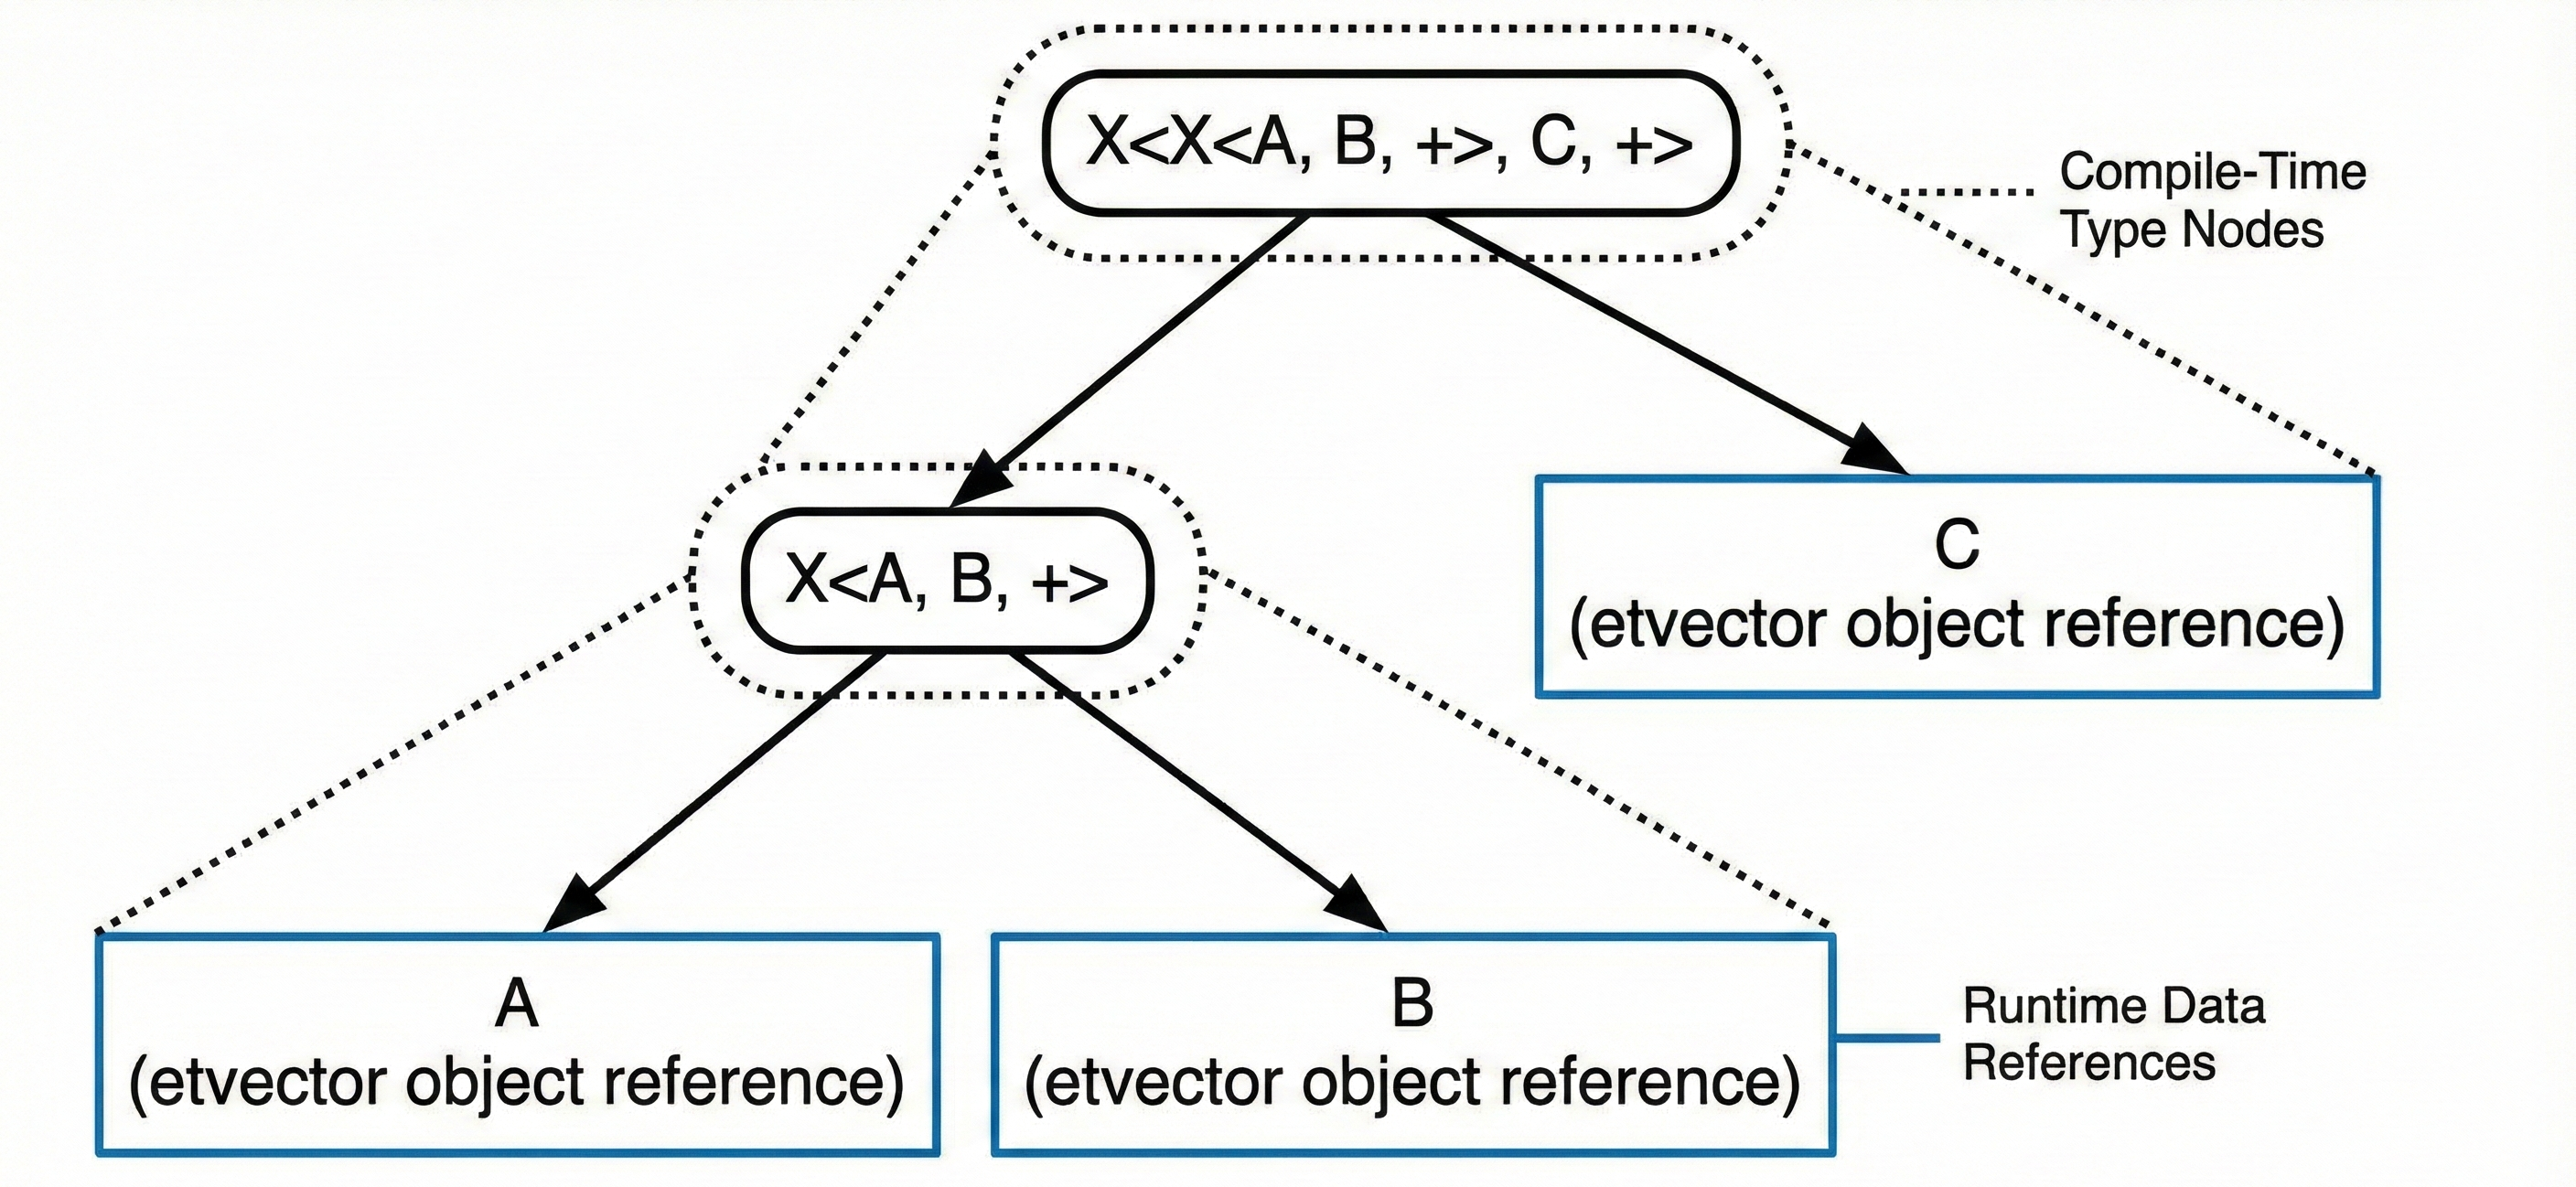
\includegraphics[width=0.6\textwidth]{placeholder_expression_template_tree.png}
\caption{Expression template type tree for \texttt{A + B + C}. Each node is an \texttt{X<Left, Right, Op>} template instantiation. Leaf nodes are \texttt{etvector} objects containing actual data. The tree exists only in the type system at compile-time; at runtime, only references and inline function calls remain.}
\end{figure}

\section{Real-World Applications: High-Performance Computing Libraries}

\subsection{Historical Context: Blitz++}

\textbf{Blitz++} was the pioneering library that popularized expression templates for scientific computing. Developed by Todd Veldhuizen (one of the inventors of the technique), it demonstrated that C++ could achieve performance competitive with Fortran---the traditional gold standard for numerical computing.

\subsubsection{Key Features of Blitz++}

\begin{itemize}
    \item \textbf{N-dimensional arrays:} \texttt{Array<T, D>} where \texttt{D} is the number of dimensions
    \begin{lstlisting}[language=C++]
    Array<double, 2> matrix(100, 100);  // 2D array
    Array<float, 3> volume(50, 50, 50);  // 3D array
    \end{lstlisting}
    
    \item \textbf{Fixed-size vectors:} \texttt{TinyVector<T, N>} for small vectors
    \begin{lstlisting}[language=C++]
    TinyVector<double, 3> position;  // 3D point
    TinyVector<float, 4> quaternion;  // Quaternion
    \end{lstlisting}
    
    \item \textbf{Expression templates:} Full support for complex mathematical expressions
    \begin{lstlisting}[language=C++]
    Array<double, 2> A, B, C;
    C = A + B * 2.0 - sin(A);  // Single-pass evaluation!
    \end{lstlisting}
    
    \item \textbf{Available today:} \url{https://github.com/blitzpp/blitz}
\end{itemize}

\subsubsection{Performance Results}

The slides include a benchmark graph showing:

\begin{figure}[h!]
\centering
\includegraphics[width=0.7\textwidth]{placeholder_blitz_performance_comparison.png}
\caption{Performance comparison of different languages/implementations for vector operations (DAXPY: \texttt{y = a*x + y}). Blitz++ achieves >90\% of Fortran 77 performance, significantly outperforming Fortran 90/95 array syntax and standard C++. Y-axis: Performance in MFlops, X-axis: Vector length. Source: Historical data from \url{http://www.oonumerics.org/blitz/benchmarks/daxpy.html}}
\end{figure}

\textbf{Key findings:}
\begin{itemize}
    \item Blitz++ TinyVector: Excellent for small vectors
    \item Blitz++ Array: Strong overall performance
    \item Fortran 77: Baseline peak performance
    \item Fortran 90/95: Surprisingly slower (overhead from array syntax)
    \item C++ valarray (standard library): Poor performance
\end{itemize}

\textbf{Significance:} This demonstrated that C++ with expression templates could match or exceed Fortran's numerical performance while providing better abstraction and type safety.

\subsection{Modern C++ Linear Algebra Libraries}

Today, expression templates are ubiquitous in high-performance C++ numerical computing. All major libraries use them:

\subsubsection{Eigen}

\textbf{Website:} \url{http://eigen.tuxfamily.org/}

\textbf{Features:}
\begin{itemize}
    \item Most popular modern C++ linear algebra library
    \item Excellent documentation and examples
    \item Highly optimized with expression templates, SIMD, and cache-aware algorithms
    \item Support for dense and sparse matrices
\end{itemize}

\textbf{Expression template insight:} See their detailed explanation at \url{http://eigen.tuxfamily.org/dox/TopicInsideEigenExample.html}

\textbf{Example:}
\begin{lstlisting}[language=C++, caption={Eigen usage with expression templates}]
#include <Eigen/Dense>
using Eigen::MatrixXd;
using Eigen::VectorXd;

MatrixXd A(3, 3);
VectorXd b(3), x(3);

// Initialize A and b...

// Solve linear system Ax = b
x = A.colPivHouseholderQr().solve(b);

// Complex expression: single-pass evaluation
VectorXd y = 2.0 * x + b.array().sin().matrix();
\end{lstlisting}

\subsubsection{Blaze}

\textbf{Website:} \url{https://bitbucket.org/blaze-lib/blaze}

\textbf{Focus:} Maximum performance through aggressive optimization

\textbf{Features:}
\begin{itemize}
    \item Expression templates with smart expression analysis
    \item Automatic kernel selection (different algorithms for different sizes)
    \item Extensive SIMD vectorization
    \item Cache optimization
\end{itemize}

\subsubsection{Armadillo}

\textbf{Website:} \url{http://arma.sourceforge.net/}

\textbf{Focus:} Matlab-like syntax with high performance

\textbf{Features:}
\begin{itemize}
    \item Intuitive API similar to Matlab
    \item Expression templates under the hood
    \item Integration with LAPACK and BLAS
    \item Good for rapid prototyping
\end{itemize}

\textbf{Example:}
\begin{lstlisting}[language=C++, caption={Armadillo usage}]
#include <armadillo>
using namespace arma;

mat A = randu<mat>(4, 5);
mat B = randu<mat>(4, 5);

// Element-wise operations with expression templates
mat C = A + 2.0 * B - 1.0;

// Linear algebra
vec eigenvalues = eig_sym(A * A.t());
\end{lstlisting}

\subsubsection{MTL4 (Matrix Template Library)}

\textbf{Website:} \url{http://www.mtl4.org}

\textbf{Focus:} Generic programming for numerical linear algebra

\textbf{Features:}
\begin{itemize}
    \item Strong emphasis on generic programming
    \item Expression templates
    \item Extensive support for different matrix formats
    \item Integration with iterative solvers
\end{itemize}

\subsubsection{Boost uBLAS}

\textbf{Website:} \url{https://www.boost.org/doc/libs/1_74_0/libs/numeric/ublas/doc/index.html}

\textbf{Focus:} Part of the Boost C++ library collection

\textbf{Features:}
\begin{itemize}
    \item Well-tested and stable
    \item Expression templates
    \item Integration with Boost ecosystem
    \item Good documentation
\end{itemize}

\subsection{Common Themes Across Libraries}

All these libraries share key characteristics:

\begin{enumerate}
    \item \textbf{Expression Templates:} Core optimization technique
    \item \textbf{Zero-Overhead Abstractions:} High-level code compiles to optimal machine code
    \item \textbf{SIMD Vectorization:} Exploitation of CPU vector instructions
    \item \textbf{Cache Optimization:} Data layout and access patterns optimized for modern CPUs
    \item \textbf{Template Metaprogramming:} Compile-time code generation and optimization
\end{enumerate}

\subsection{Choosing a Library}

\textbf{For general use:} Eigen (excellent documentation, widely used)

\textbf{For maximum performance:} Blaze (aggressive optimization)

\textbf{For Matlab users:} Armadillo (familiar syntax)

\textbf{For generic programming:} MTL4 (flexible, extensible)

\textbf{For Boost users:} uBLAS (integrated ecosystem)

\section{Advanced Applications: Beyond Vector Operations}

\subsection{Automatic Differentiation with Expression Templates}

Expression templates can do more than optimize evaluation---they can \textit{transform} expressions. One powerful application is automatic differentiation.

\subsubsection{The Concept}

Consider the expression:
\begin{equation}
f(x) = 3(x + 1) + 4
\end{equation}

With expression templates, this creates a type structure:
\begin{lstlisting}[language=C++, caption={Expression template type for differentiation}]
Expression
    <Expression< Constant<int>,                      // 3
            Expression< Variable,
                        Constant<int>,
                        Add>,  // x + 1
            Multiply >,
    Constant<int>,                          // 4
    Add >
\end{lstlisting}

This type represents the expression tree:
\begin{verbatim}
         +
       /   \
      *     4
     / \
    3   +
       / \
      x   1
\end{verbatim}

\subsubsection{Compile-Time Differentiation}

Since the expression tree exists in the type system, we can write template metaprograms that:

\begin{itemize}
    \item \textbf{Compute derivatives:} Apply differentiation rules to the type structure
    \begin{equation}
    \frac{d}{dx}[3(x + 1) + 4] = 3 \cdot \frac{d}{dx}[x + 1] = 3 \cdot 1 = 3
    \end{equation}
    
    \item \textbf{Simplify expressions:} Constant folding, algebraic simplification
    \begin{itemize}
        \item $0 + x \rightarrow x$
        \item $1 \cdot x \rightarrow x$
        \item $x - x \rightarrow 0$
    \end{itemize}
    
    \item \textbf{Generate optimized evaluation code:} Specialized code paths based on expression structure
\end{itemize}

\subsubsection{Implementation Sketch}

\begin{lstlisting}[language=C++, caption={Basic structure for automatic differentiation}]
template <typename T> 
class Constant {
    T value_;
public:
    explicit Constant(T v) : value_(v) {}
    T eval() const { return value_; }
    Constant<int> derive() const { return Constant<int>(0); }  // d/dx[c] = 0
};

template <typename T> 
class Variable {
public:
    T eval(T x) const { return x; }
    Constant<int> derive() const { return Constant<int>(1); }  // d/dx[x] = 1
};

enum OP_enum {Add, Multiply};

template<typename L, typename R, OP_enum op>
class Expression {
    L left_;
    R right_;
public:
    Expression(const L& l, const R& r) : left_(l), right_(r) {}
    
    auto eval(auto x) const {
        if constexpr (op == Add) {
            return left_.eval(x) + right_.eval(x);
        } else if constexpr (op == Multiply) {
            return left_.eval(x) * right_.eval(x);
        }
    }
    
    auto derive() const {
        if constexpr (op == Add) {
            // d/dx[f + g] = f' + g'
            return Expression<decltype(left_.derive()), decltype(right_.derive()), Add>(
                left_.derive(), right_.derive()
            );
        } else if constexpr (op == Multiply) {
            // d/dx[f * g] = f' * g + f * g'
            // (Simplified version)
            // ...
        }
    }
};
\end{lstlisting}

This is a simplified sketch. Real automatic differentiation libraries are more sophisticated, but they use these principles.

\subsubsection{Real-World AD Libraries}

\begin{itemize}
    \item \textbf{Adept:} Automatic differentiation using expression templates
    \item \textbf{CppAD:} C++ algorithmic differentiation
    \item \textbf{Stan Math Library:} Used in Bayesian inference
\end{itemize}

\subsection{Domain-Specific Languages (DSLs)}

Expression templates enable embedding domain-specific languages in C++:

\begin{itemize}
    \item \textbf{Boost.Spirit:} Parser framework using expression templates to describe grammars
    \item \textbf{Boost.Proto:} Library for building DSLs with expression templates
    \item \textbf{Tensor networks:} Expressing quantum computations
\end{itemize}

\section{Practical Considerations and Best Practices}

\subsection{When to Use Expression Templates}

\textbf{Good use cases:}
\begin{itemize}
    \item Vector and matrix operations
    \item Complex numerical expressions evaluated many times
    \item Performance-critical code where temporaries are expensive
    \item Domain-specific languages
\end{itemize}

\textbf{Not ideal for:}
\begin{itemize}
    \item Operations performed only once
    \item Cases where code complexity outweighs performance gains
    \item When compile times become prohibitive
\end{itemize}

\subsection{Compilation Time Concerns}

Expression templates can significantly increase compilation time:

\begin{itemize}
    \item Complex type names
    \item Many template instantiations
    \item Potentially exponential growth in template depth
\end{itemize}

\textbf{Mitigation strategies:}
\begin{itemize}
    \item Use explicit instantiation for common types
    \item Employ compilation firewalls (pimpl idiom)
    \item Use precompiled headers
    \item Modern compilers are better at managing this
\end{itemize}

\subsection{Error Messages}

Template errors can be cryptic:

\begin{verbatim}
error: no match for 'operator=' (operand types are 
'etvector<double>' and 'X<X<etvector<double>, 
etvector<double>, plus>, X<etvector<double>, 
etvector<double>, minus>, multiplies>')
\end{verbatim}

\textbf{Strategies for readable errors:}
\begin{itemize}
    \item Use type aliases (\texttt{using}) to simplify types
    \item Employ concepts (C++20) to provide better diagnostics
    \item Use static assertions with clear messages
    \item Compilers are improving error messages for templates
\end{itemize}

\subsection{Debugging}

Debugging optimized expression template code can be challenging:

\begin{itemize}
    \item Compiler optimizations make single-stepping difficult
    \item Expression trees are compile-time constructs
\end{itemize}

\textbf{Approaches:}
\begin{itemize}
    \item Compile without optimization (\texttt{-O0}) for debugging
    \item Use \texttt{static\_assert} to verify type properties
    \item Write unit tests for small expressions
    \item Use tools like C++ Insights to visualize generated code
\end{itemize}

\subsection{Aliasing Issues}

Be careful with aliasing (when operands and results overlap):

\begin{lstlisting}[language=C++, caption={Potential aliasing problem}]
etvector<double> a(N);
a = a + a;  // Safe: each a[i] read before written

etvector<double> b(N);
b = b + b[0];  // Potentially problematic if b[0] changes during evaluation
\end{lstlisting}

Most libraries handle this correctly, but be aware of potential issues.

\section{Advanced Topics: C++11/14/17/20 Enhancements}

\subsection{constexpr Functions (C++11/14/17)}

Modern C++ provides \texttt{constexpr} functions, which can execute at compile time:

\begin{lstlisting}[language=C++, caption={Compile-time factorial with constexpr}]
constexpr int factorial(int n) {
    return (n <= 1) ? 1 : n * factorial(n - 1);
}

// Computed at compile time
constexpr int result = factorial(5);  // result = 120

// Can be used as template parameter
std::array<int, factorial(4)> arr;  // Array of size 24
\end{lstlisting}

This is often simpler than template metaprogramming for numerical computations.

\subsection{Variable Templates (C++14)}

\begin{lstlisting}[language=C++, caption={Variable templates for constants}]
template<typename T>
constexpr T pi = T(3.1415926535897932385);

double area = pi<double> * r * r;
float circumference = 2.0f * pi<float> * r;
\end{lstlisting}

\subsection{Fold Expressions (C++17)}

Simplify recursive template patterns:

\begin{lstlisting}[language=C++, caption={Fold expressions for variadic templates}]
template<typename... Args>
auto sum(Args... args) {
    return (... + args);  // Fold expression
}

int result = sum(1, 2, 3, 4, 5);  // result = 15
\end{lstlisting}

\subsection{Concepts (C++20)}

Concepts provide constraints on templates with clear error messages:

\begin{lstlisting}[language=C++, caption={Concepts for better template constraints}]
template<typename T>
concept Numeric = std::is_arithmetic_v<T>;

template<Numeric T>
T add(T a, T b) {
    return a + b;
}

// Clear error if called with non-numeric type
// add(std::string("a"), std::string("b"));  // Error: constraint not satisfied
\end{lstlisting}

\subsection{Ranges and Views (C++20)}

The ranges library provides lazy evaluation for standard algorithms:

\begin{lstlisting}[language=C++, caption={C++20 ranges with lazy evaluation}]
#include <ranges>
#include <vector>

std::vector<int> vec = {1, 2, 3, 4, 5};

// Lazy evaluation: no intermediate vectors created
auto result = vec 
    | std::views::transform([](int x) { return x * 2; })
    | std::views::filter([](int x) { return x > 5; })
    | std::views::take(2);

for (int x : result) {
    std::cout << x << '\n';  // 6, 8
}
\end{lstlisting}

This uses expression template-like techniques internally.

\section{Conclusion: The Power of Zero-Cost Abstractions}

\subsection{Key Takeaways}

Throughout this chapter, we've explored a suite of advanced C++ optimization techniques:

\begin{enumerate}
    \item \textbf{Inlining:} Eliminates function call overhead, enabling secondary optimizations
    
    \item \textbf{Copy Elision/RVO/NRVO:} Compiler optimizations that eliminate unnecessary object copies
    
    \item \textbf{Template Metaprogramming:} Moves computation from runtime to compile time
    
    \item \textbf{Loop Unrolling:} Uses template recursion to eliminate loop overhead for fixed-size operations
    
    \item \textbf{Lazy Evaluation:} Postpones computation until results are needed
    
    \item \textbf{Expression Templates:} Combines templates with lazy evaluation to optimize complex expressions
\end{enumerate}

\subsection{The Philosophy of Zero-Cost Abstractions}

These techniques exemplify C++'s core philosophy: \textbf{"what you don't use, you don't pay for"} and \textbf{"what you do use, you couldn't hand code any better."} 

Expression templates allow us to write:
\begin{lstlisting}[language=C++]
vector a = b + c + d;  // Elegant, mathematical
\end{lstlisting}

While generating code equivalent to:
\begin{lstlisting}[language=C++]
for (int i = 0; i < N; ++i) {
    a[i] = b[i] + c[i] + d[i];  // Optimal, hand-written
}
\end{lstlisting}

\textbf{We get both abstraction and performance!}

\subsection{Broader Impact}

These techniques have enabled:

\begin{itemize}
    \item C++ to compete with Fortran in numerical computing
    \item Development of sophisticated scientific simulation software
    \item High-performance game engines
    \item Financial modeling systems
    \item Machine learning frameworks
    \item Real-time graphics and physics
\end{itemize}

\subsection{Looking Forward}

Modern C++ (C++11 and beyond) continues to evolve:

\begin{itemize}
    \item \texttt{constexpr} functions simplify compile-time computation
    \item Concepts improve template error messages
    \item Ranges provide standard library support for lazy evaluation
    \item Modules may improve compilation times
\end{itemize}

However, the fundamental techniques---templates, inlining, and compile-time code generation---remain central to high-performance C++ programming.

\subsection{Final Thoughts}

Understanding these optimization techniques is essential for anyone working on performance-critical C++ code, especially in scientific computing. They represent decades of evolution in compiler technology and programming language design.

The beauty of these approaches is that they make the compiler work for you. By structuring code appropriately, you enable the compiler to generate optimal machine code automatically. This is the essence of modern C++ programming: writing clear, maintainable code that compiles to efficient executables.

As you develop your own scientific simulation code, consider:
\begin{itemize}
    \item When to use existing libraries (Eigen, Blaze, etc.) vs. implement custom solutions
    \item Where performance bottlenecks actually exist (measure first!)
    \item The trade-offs between code complexity and performance gains
    \item How these techniques can be combined with other optimizations (SIMD, cache optimization, parallelization)
\end{itemize}

Master these techniques, and you'll be equipped to write C++ code that is both elegant and blazingly fast---truly achieving the ideal of zero-cost abstractions.

\section{Appendix: Further Resources and References}

\subsection{Key Papers and Publications}

\begin{itemize}
    \item Todd Veldhuizen, "Expression Templates," \textit{C++ Report}, June 1995
    \item Todd Veldhuizen, "Techniques for Scientific C++," Indiana University Computer Science Technical Report \#542, 2000
    \item David Vandevoorde and Nicolai M. Josuttis, \textit{C++ Templates: The Complete Guide}, Addison-Wesley
    \item Erwin Unruh, "Prime Number Computation" (1994), \url{http://www.erwin-unruh.de/Prim.html}
\end{itemize}

\subsection{Online Resources}

\begin{itemize}
    \item \textbf{cppreference.com}: Comprehensive C++ reference
    \begin{itemize}
        \item Inline: \url{https://en.cppreference.com/w/cpp/language/inline}
        \item Copy elision: \url{https://en.cppreference.com/w/cpp/language/copy_elision}
        \item Evaluation order: \url{https://en.cppreference.com/w/cpp/language/eval_order}
        \item Operator precedence: \url{https://en.cppreference.com/w/cpp/language/operator_precedence}
    \end{itemize}
    
    \item \textbf{C++ Insights}: \url{https://cppinsights.io/} - See what the compiler generates from your templates
    
    \item \textbf{Compiler Explorer}: \url{https://godbolt.org/} - View assembly output for different compilers and optimization levels
\end{itemize}

\subsection{Library Documentation}

\begin{itemize}
    \item \textbf{Eigen}: \url{http://eigen.tuxfamily.org/}
    \item \textbf{Blaze}: \url{https://bitbucket.org/blaze-lib/blaze}
    \item \textbf{Armadillo}: \url{http://arma.sourceforge.net/}
    \item \textbf{MTL4}: \url{http://www.mtl4.org}
    \item \textbf{Boost uBLAS}: \url{https://www.boost.org/doc/libs/1_74_0/libs/numeric/ublas/doc/index.html}
    \item \textbf{Blitz++}: \url{https://github.com/blitzpp/blitz}
\end{itemize}

\subsection{Books for Further Study}

\begin{itemize}
    \item Bjarne Stroustrup, \textit{The C++ Programming Language} (4th Edition)
    \item Scott Meyers, \textit{Effective Modern C++}
    \item Andrei Alexandrescu, \textit{Modern C++ Design}
    \item David Vandevoorde, Nicolai M. Josuttis, Douglas Gregor, \textit{C++ Templates: The Complete Guide} (2nd Edition)
\end{itemize}

\subsection{Courses and Tutorials}

\begin{itemize}
    \item CppCon conference talks (YouTube)
    \item C++Now conference talks
    \item Coursera and edX courses on C++ and parallel programming
    \item LearnCpp.com online tutorial
\end{itemize}

\end{document}
